\documentclass[tikz,border=3mm]{standalone}
\usetikzlibrary{calc,patterns,arrows.meta}

\begin{document}
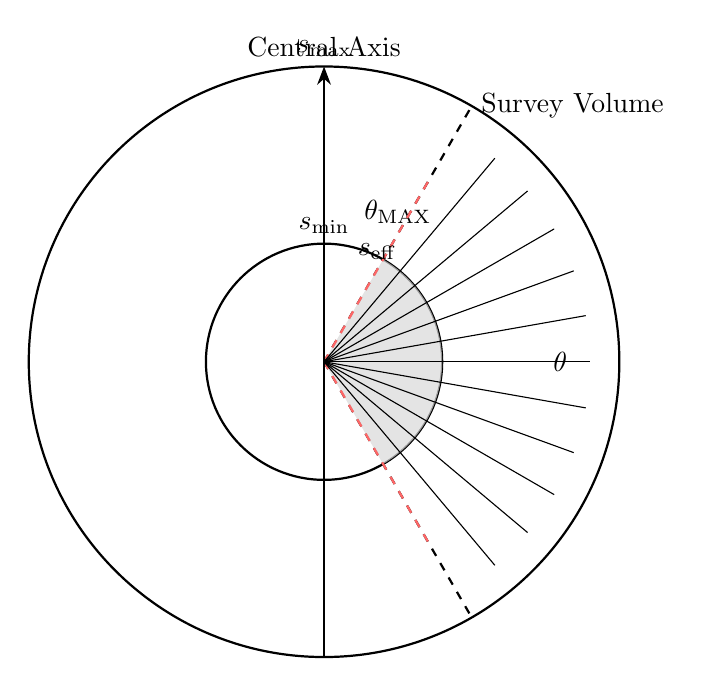
\begin{tikzpicture}[>=Stealth,scale=1.5]
    % Parameters
    \def\smin{1.0}
    \def\smax{2.5}
    \def\seff{1.8}
    \def\thetaMAX{60} % Angular opening in degrees

    % Coordinate system
    \coordinate (O) at (0,0);
    \coordinate (N) at (0,\smax);
    \coordinate (S) at (0,-\smax);

    % Draw outer boundary (s_max)
    \draw[thick] (O) circle (\smax);
    % Draw inner boundary (s_min)
    \draw[thick] (O) circle (\smin);

    % Angular sector (theta_MAX)
    \draw[thick,dashed] (O) -- ++(\thetaMAX:\smax) node[midway,above] {$\theta_\mathrm{MAX}$};
    \draw[thick,dashed] (O) -- ++(-\thetaMAX:\smax);

    % Shade survey volume
    \begin{scope}
        \clip (O) -- ++(\thetaMAX:\smax) arc (\thetaMAX:-\thetaMAX:\smax) -- (O);
        \clip (O) -- ++(\thetaMAX:\smin) arc (\thetaMAX:-\thetaMAX:\smin) -- (O);
        \fill[gray!30,opacity=0.7] (O) circle (\smax);
    \end{scope}

    % Effective distance (s_eff)
    \draw[dashed,thick,red!60] (O) -- ++(\thetaMAX:\seff) node[midway,above,black] {$s_\mathrm{eff}$};
    \draw[dashed,thick,red!60] (O) -- ++(-\thetaMAX:\seff);

    % Labels
    \node at (0,\smax) [above] {$s_\mathrm{max}$};
    \node at (0,\smin) [above] {$s_\mathrm{min}$};
    \node at (\thetaMAX:\smax) [right] {Survey Volume};

    % Central axis
    \draw[->,thick] (S) -- (N) node[above] {Central Axis};

    % Angular scale
    \foreach \angle in {-50,-40,...,50} {
        \draw[thin] (O) -- ++(\angle:\smax*0.9);
    }
    \node at (0:\smax*0.8) {$\theta$};
\end{tikzpicture}
\end{document}